\documentclass[hyperref={pdfpagelabels=false}]{beamer}
\usepackage{beamerthemesplit}
\usepackage{lmodern}
\title{Using linux at UIC}
\author{UIC Linux Users Group}
\date{\today}
\begin{document}
\frame{\titlepage}
\section{Wireless}
\subsection{About 802.1x}
\frame
{
    \frametitle{802.1x (Dynamic WEP)}
    \begin{itemize}
    \item{Wireless security mechanism designed to address shortcomings in previous wireless security schemes.}
    \item{Per user Authentication}
    \item{implemented before wpa2}
    \end{itemize}
}
\subsection{Network Manager}
\frame
{
    \frametitle{Network Manager}
    
    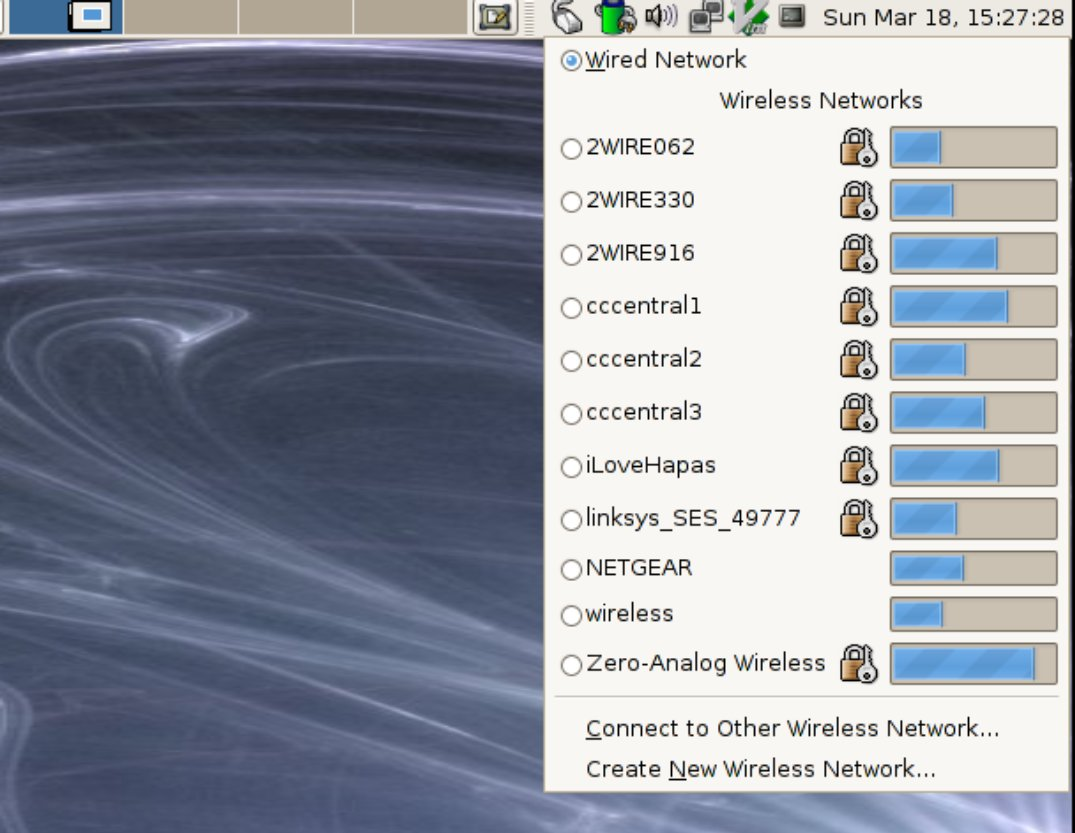
\includegraphics[totalheight=0.7\textheight]{gnm.jpg}

}
\frame
{
    \frametitle{connecting to the network}
    http://acm.cs.uic.edu/uicwireless-linux

    security: dynamic wep (802.1x)
}
\subsection{Wireless Settings}
\frame
{
     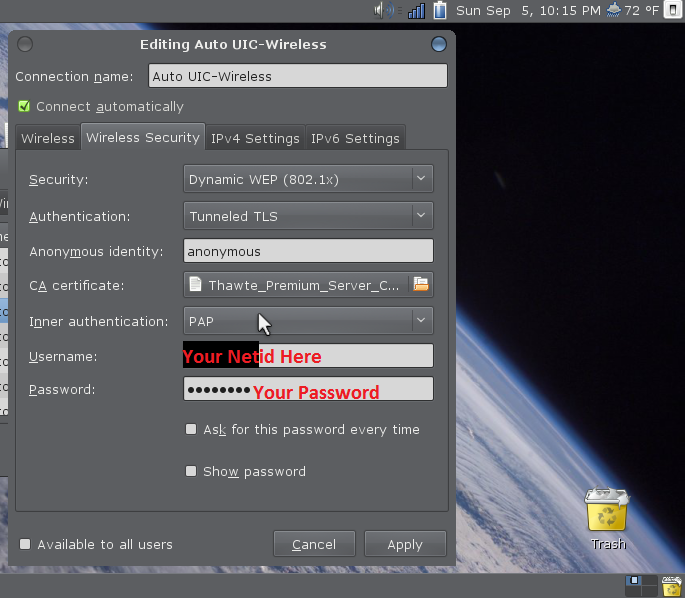
\includegraphics[totalheight=0.8\textheight]{uicwirelessstep2.png}
}
\frame
{
    \frametitle{network settings}
    \begin{itemize}
    \item{Network name: UIC-Wireless}
    \item{Wireless Security: Dynamic WEP (802.1x)}
    \item{Authentication: Tunneled TLS}
    \item{Anonymous Identity: anonymous}
    \item{inner Authentication: PAP}
    \item{Username: ACCC NETID}
    \item{Password: ACCC PASSWORD}
    \end{itemize}
}
\frame
{
    \frametitle{Pray}
    Pray...
}
\section{Printing}
\subsection{Pharos}
\frame
{
    \frametitle{Pharos}
    Pharos is ACCC's print management system at UIC.
}
\subsection{Setup}
\frame
{
    \frametitle{Setup}
     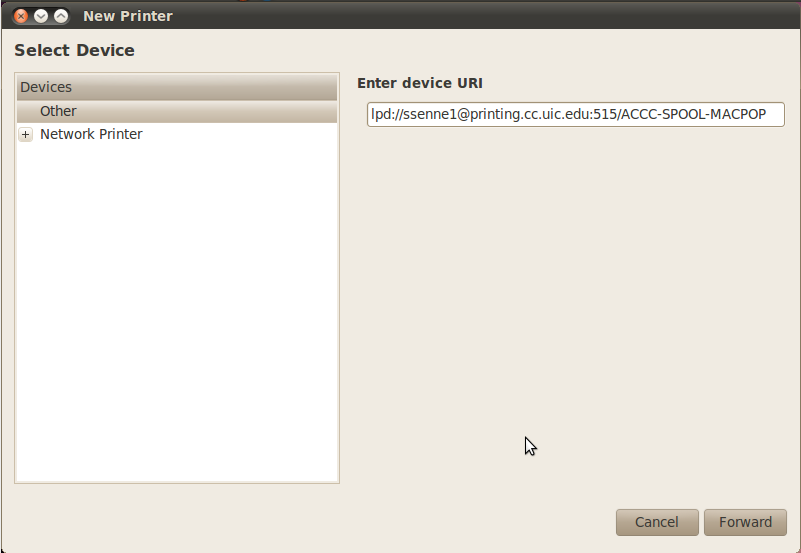
\includegraphics[totalheight=0.8\textheight]{PrinterURI.png}
}
\subsection{Select Printer Driver}
\frame
{
    \frametitle{Select Printer Driver}
     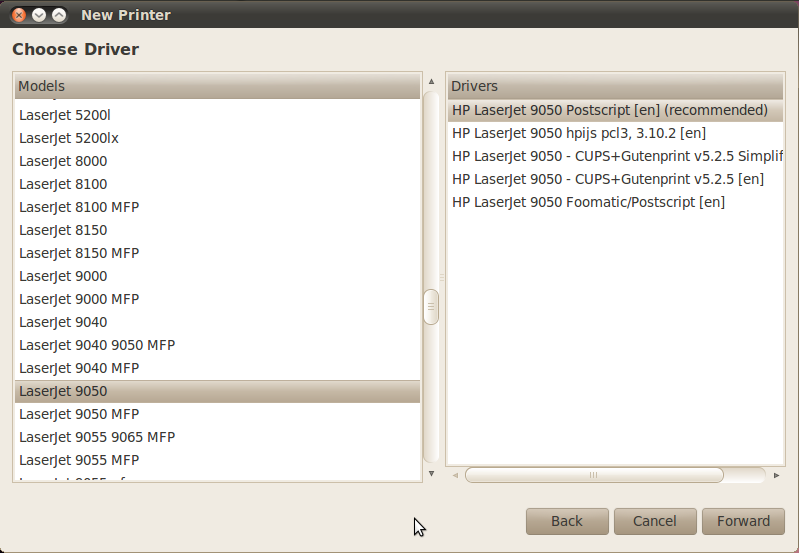
\includegraphics[totalheight=0.8\textheight]{PrinterDriver.png}
}
\frame
{
    \frametitle{Name Printer}
     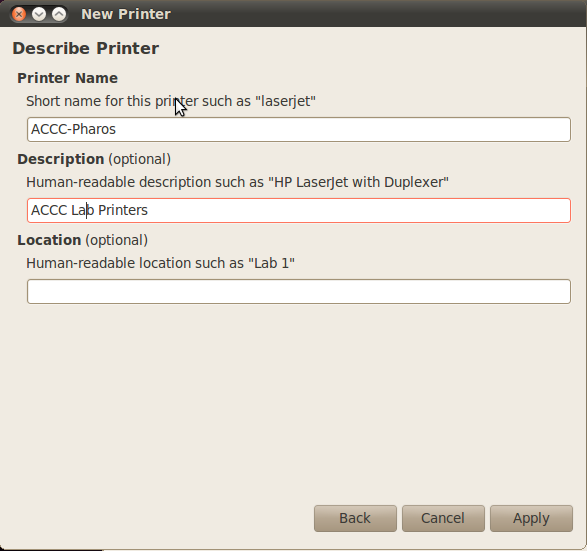
\includegraphics[totalheight=0.8\textheight]{PrinterName.png}

}
\subsection{Summary}
\frame
{
    \frametitle{Summary}
URI: lpd://NETID@printing.cc.uic.edu:515/ACCC-SPOOL-MACPOP\\
Select printer from database: HP LaserJet 9050 Postscript \[en\]
Select Duplex \(if you want\)
}
\section{Turnin}
\subsection{What is Turnin}
\frame
{
    \frametitle{What is turnin}
    turnin is a a unix program for turning in CS programing assignments.
}

\subsection{Features}
\frame
{
    \frametitle{Features of Turnin}
    \begin{itemize}
    \item{Verify that your program was turned in successfully}
    \item{turn in asignment multiple times (until the deadline)}
    \end{itemize}
}
\subsection{Usage}
\subsection{Finding Assingments}
\frame
{
    \frametitle{Checking the List of Assignments}
	turnin -c cs102 -l
}
\subsection{Turning in an Assignment}
\frame
{
    \frametitle{Turning in an Assignment}
	turnin -c cs102 -p prog1 myfile\\
	turnin -c cs102 -p prog1 MyProjectFolder\\
	turnin -c cs102 -p prog1 *.java
}
\subsection{Verifying Turnin}
\frame
{
    \frametitle{Ensureing That an Assigment Was Turned In}
	turnin -c cs102 -p prog1 -v

}
\subsection{Resubmitting an Assingment}
\frame
{
    \frametitle{Turning in an Assignment a Second Time}
	turnin -c cs102 -p prog1 myfile\\
	turnin -c cs102 -p prog1 MyProjectFolder\\
	turnin -c cs102 -p prog1 *.java\\
	
}
\section{UIC Servers}
\frame
{
    \frametitle{UIC Servers}
    2 campus departments manage servers we have access to: ACCC and the CS department.
}
\subsection{Icarus}
\frame
{
    \frametitle{icarus.uic.edu}
    \begin{itemize}
    \item{ACCC server}
    \item{web hosting}
    \item{php, perl, bluestem, html}
    \item{shell access}
    \item{http://www2.uic.edu/$\sim$netid/}
    \item{Solaris}
    \end{itemize}
}
\subsection{Bert}
\frame
{
    \frametitle{Bert}
    \begin{itemize}
    \item{CS Department Server}
    \item{html}
    \item{Web hosting}
    \item{http://cs.uic.edu/$\sim$cslogin/}
    \item{RHEL 5.5}
    \end{itemize}
}
\subsection{Webspace}
\frame
{
    \frametitle{How to use webspace}
    \begin{itemize}
    \item{create a $\sim$/public\_hmtl directory}
    \end{itemize}
}
\section{Getting Help}

\subsection{ACCC}
\frame
{
	\frametitle{ACCC}
	The ACCC officially does not support linux, and will usually turn you away if
	seek assistance from them.
}
\frame
{
    \frametitle{Issues with ACCC}
    \begin{itemize}
    \item{ACCC account trouble}
    \item{windows/mac labs}
    \item{uic email}
    \item{wireless/resnet}
    \end{itemize}
}
\subsection{Contacting ACCC}
\frame
{
    \frametitle{Contacting ACCC}
    \begin{itemize}
    \item{talk to any ACCC consultant or lab monitor}
    \item{support@uic.edu}
    \item{312-413-0003}
    \end{itemize}
}
\subsection{CS Department}
\frame
{
    \frametitle{Issues with CS department Computers}
    \begin{itemize}
    \item{If you don't know your account info}
    \item{If you your account info doesn't work}
    \item{If you need help using software}
    \item{If you need software installed for a class.}
    \end{itemize}
}
\subsection{Contacting CS Department}
\frame
{
    \frametitle{Contacting CS department}
    \begin{itemize}
    \item{pester Stephen Liang}

    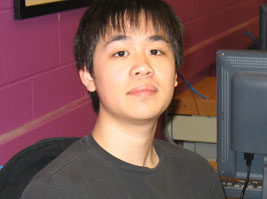
\includegraphics[totalheight=0.3\textheight]{sliang6.jpg}
    \item{email support@cs.uic.edu}
    \end{itemize}
}
\end{document}
v
